\section{Design Front-End}
In questo capitolo si presenta un prototipo semplificato dell'applicazione. In ogni schermata sono stati integrati e garantiti dei requisiti non funzionali come:
\begin{itemize}
    \item \textbf{RF0: Localizzazione}
    \begin{itemize}
        \item È sempre garantita la possibilità di selezionare la lingua dell'interfaccia (italiano, inglese o tedesco): nelle schermate di accesso è presente il selettore tramite bandiera, mentre all'interno dell'applicativo è stato integrato il comando dedicato nella barra laterale (icona multilingua), permettendo la persistenza delle preferenze dell'utente.
    \end{itemize}
    \item \textbf{RNF1: Compatibilità}
    \begin{itemize}
        \item L'interfaccia è progettata come applicazione web, compatibile con i principali browser (Firefox, Chrome, Edge, Safari) e fruibile anche su dispositivi tablet con schermo minimo di 10 pollici.
    \end{itemize}

    \item \textbf{RNF5: Sicurezza}
    \begin{itemize}
        \item La sicurezza del sistema si riflette nell'adozione del protocollo cifrato HTTPS per ogni interazione client-server, nell'oscuramento delle credenziali riservate e nell'implementazione di controlli di validazione dei campi di input. Inoltre, l'interfaccia implementa la divisione dei ruoli (Role-Based Access Control), mostrando elementi di navigazione e azioni critiche (ad esempio la gestione utenti o le impostazioni avanzate) esclusivamente agli utenti che hanno i privilegi di amministratore.
    \end{itemize}
    
    \item \textbf{RNF6: Usabilità}
    \begin{itemize}
        \item L'interfaccia adotta un layout semplice e coerente in ogni sezione, caratterizzato da una barra di navigazione laterale fissa con icone universali (Dashboard, Mappa, Edifici, Sensori, Allarmi e per gli amministratori anche le interfacce Utenti e Impostazioni). I componenti visivi (schede di riepilogo, campi di input ed etichette esplicative) sono stati scelti per garantire un apprendimento rapido e minimizzare il rischio di errore umano.
    \end{itemize}

    \item \textbf{RNF7: Conformità normativa (Accessibilità)}
    \begin{itemize}
        \item Gli elementi grafici, la disposizione degli spazi e il contrasto tra testi e sfondi sono stati impostati tenendo conto dei criteri di accessibilità WCAG 2.1 a livello A, assicurando piena leggibilità e fruibilità.
    \end{itemize}
    
\end{itemize}
\newpage
\subsection{Schermata di Login}
La schermata di login di WattGuard presenta un'interfaccia essenziale e intuitiva, studiata per ridurre le barriere all'accesso e guidare l'utente alle funzionalità della piattaforma in base ai propri privilegi.

\begin{figure}[H]
    \centering
    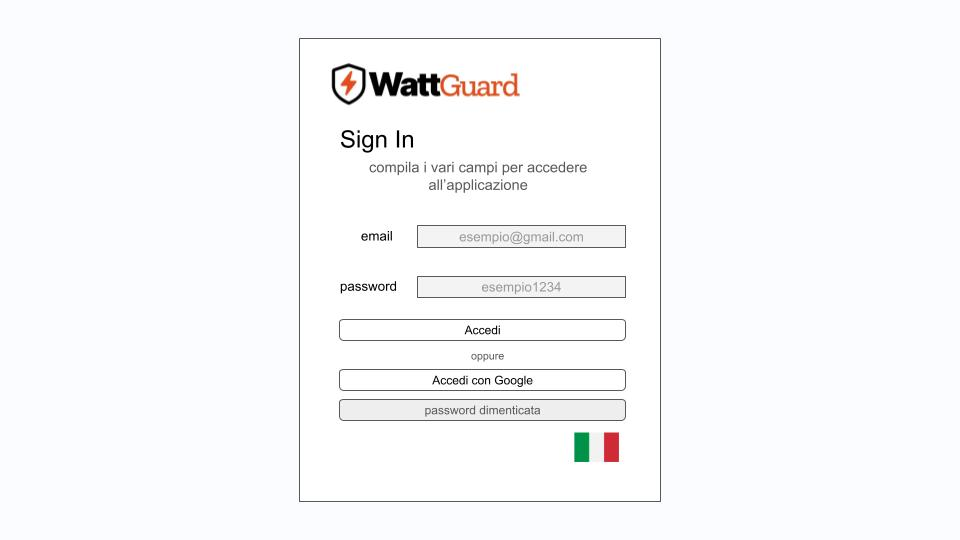
\includegraphics[width=1\textwidth]{../images/Interfaccia_grafica/Login.jpg}
    \caption{Schermata di Login}
    \label{fig:login}
\end{figure}

La Figura~\ref{fig:login} mostra il mockup della pagina di autenticazione iniziale, accessibile pubblicamente prima dell'ingresso nel sistema.

\begin{itemize}
    \item \textbf{RF1: Login}
    \begin{itemize}
        \item L'interfaccia supporta la doppia modalità di accesso: tramite credenziali locali registrate nel sistema (campi ``email'' e ``password'' con placeholder guida) o mediante autenticazione federata con il pulsante dedicato ``Accedi con Google''. 
        Attraverso l'autenticazione il sistema reindirizzerà l'utente alla dashboard generale.
        \item Nella parte inferiore è presente il pulsante ``password dimenticata'', che funge da flusso alternativo reindirizzando l'utente alla schermata di recupero delle credenziali.
    \end{itemize}
\end{itemize}
\newpage

\subsection{Schermata di Reset Password}
La schermata di reset password di WattGuard completa il flusso di autenticazione, offrendo un percorso semplice e sicuro per il recupero dell'accesso al sistema.

\begin{figure}[H]
    \centering
    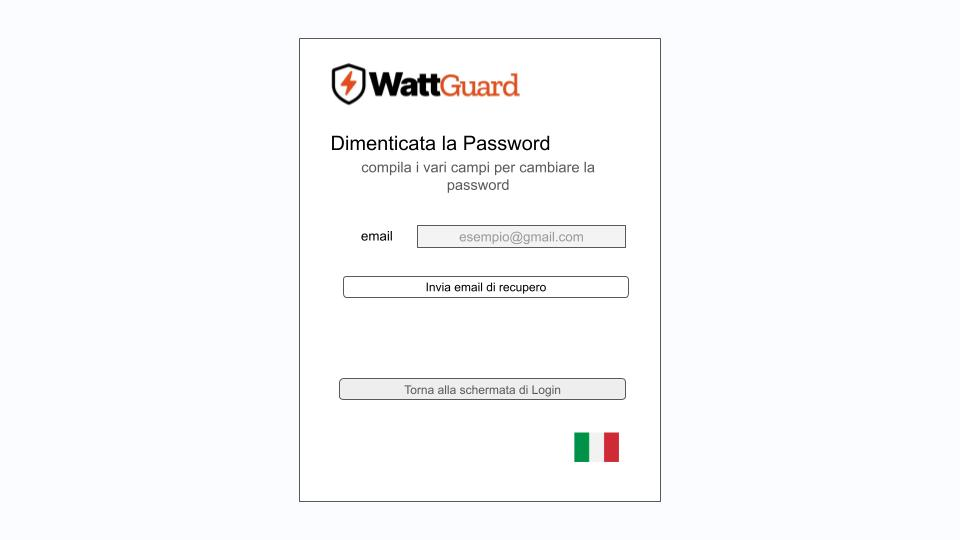
\includegraphics[width=1\textwidth]{../images/Interfaccia_grafica/Recupero_Password.jpg}
    \caption{Schermata di Reset Password}
    \label{fig:reset_password}
\end{figure}

La Figura~\ref{fig:reset_password} mostra il mockup della schermata per il recupero delle credenziali di accesso.

\begin{itemize}
    \item \textbf{RF1: Recupero credenziali}
    \begin{itemize}
        \item  La schermata consente all'utente di avviare la procedura di reset della password inserendo il proprio indirizzo email. Il sistema, una volta ricevuta la richiesta, invierà all'indirizzo indicato un link per la reimpostazione della password, in conformità con il flusso di autenticazione sicura previsto da RF1.
    \end{itemize}

    \item \textbf{RF11: Gestione utenti e credenziali}
        \begin{itemize}
            \item Il meccanismo di reset password è strettamente correlato alla gestione degli account utente. L'operatore tecnico che riceve le credenziali temporanee alla creazione dell'account può utilizzare questo flusso per impostare una nuova password al primo accesso o in caso di smarrimento.
        \end{itemize}
\end{itemize}
\newpage
\subsection{Dashboard Generale}
\begin{figure}[H]
    \centering
    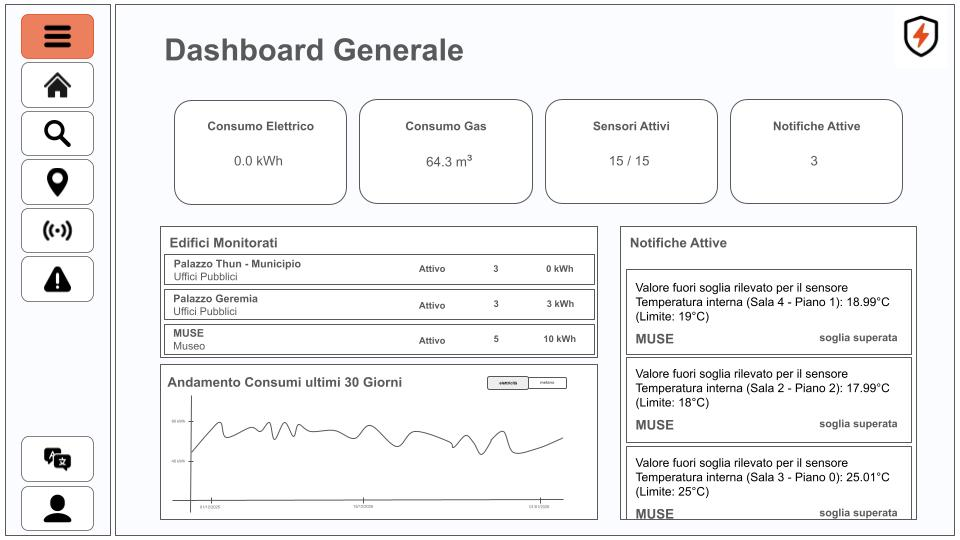
\includegraphics[width=1\textwidth]{../images/Interfaccia_grafica/Dashboard.jpg}
    \caption{Dashboard Generale del Sistema}
    \label{fig:dashboard_generale}
\end{figure}

La Figura~\ref{fig:dashboard_generale} mostra la schermata principale dell'applicazione, concepita per fornire sia all'operatore tecnico che all'amministratore una visione d'insieme immediata sullo stato energetico e operativo del patrimonio edilizio comunale.

\begin{itemize}
    \item \textbf{RF2: Visualizzazione dashboard generale}
    \begin{itemize}
        \item Nella parte superiore della schermata sono evidenziati quattro principali indicatori del sistema: Il Consumo Elettrico (in kWh), il Consumo Gas (in $\text{m}^3$), il rapporto  tra sensori attivi e sensori registrati (Sensori Attivi ) e il conteggio delle Notifiche Attive. 
        
        La vista centrale presenta il grafico storico interattivo ("Andamento Consumi ultimi 30 Giorni"). Esso mostra sia l'andamento dei consumi della corrente elettrica, sia quelli del consumo di gas. Infine la tabella riassuntiva degli "Edifici Monitorati" riporta brevemente lo stato operativo dell'edificio, numero di sensori installati e l'eventuale consumo istantaneo di corrente elettrica.
    \end{itemize}

    \item \textbf{RF6: Gestione notifiche di allarme}
    \begin{itemize}
        \item È presente una sezione dedicata alle "Notifiche Attive" che elenca in tempo reale le ultime anomalie rilevate dal sistema. Per ogni allerta vengono mostrati l'edificio coinvolto (es. MUSE), le informazioni specifiche del sensore, (es. temperatura interna in Sala 4 al Piano 1), il valore rilevato dallo stesso ($18.99\,^\circ\text{C}$) e la soglia limite impostata ($19\,^\circ\text{C}$).
        Ciò rende evidenti eventuali problemi rilevati, permettendo di agire tempestivamente sulle criticità.
    \end{itemize}

    \item \textbf{RF7: Visualizzazione stato sensori}
    \begin{itemize}
        \item La scheda di riepilogo "Sensori Attivi (15/15)" e la colonna dedicata nella tabella degli edifici consentono di monitorare quanti sensori sono attivi in un determinato momento, permettendo così di verificare a colpo d'occhio la corretta operatività dell'intera rete di rilevamento.
    \end{itemize}
    \newpage
    \item \textbf{RF8: Monitoraggio in tempo reale (visione d'insieme)}
    \begin{itemize}
        \item I KPI complessivi e le letture di consumo per singolo edificio (es. Palazzo Thun a 0\,kWh, Palazzo Geremia a 3\,kWh, MUSE a 10\,kWh) riflettono i dati telemetrici istantanei aggiornati continuamente dal meccanismo di polling.
    \end{itemize}

    \item \textbf{RNF2: Performance}
    \begin{itemize}
        \item La composizione modulare dei widget è ingegnerizzata per soddisfare il requisito di caricamento dell'intera panoramica entro 10 secondi nel 95\% dei casi, mantenendo la generazione e la resa del grafico storico a 30 giorni ampiamente sotto i 20 secondi previsti dalle specifiche.
    \end{itemize}
\end{itemize}
\newpage
\subsection{Dashboard Dettaglio Edificio}
\begin{figure}[H]
    \centering
    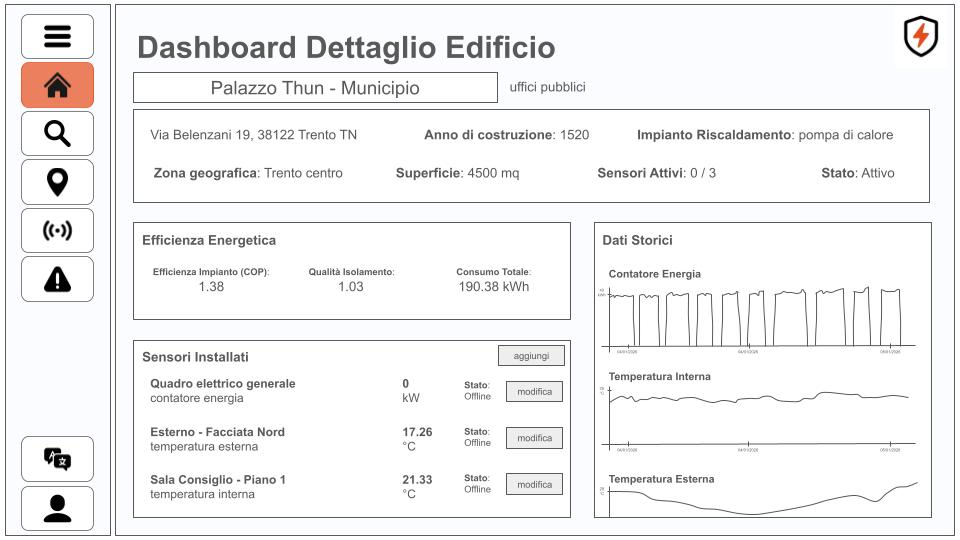
\includegraphics[width=\textwidth]{../images/Interfaccia_grafica/Pannello_Dettaglio.jpg}
    \caption{Dashboard Dettaglio Edificio}
    \label{fig:dettaglio_edificio}
\end{figure}

La Figura~\ref{fig:dettaglio_edificio} mostra il mockup della schermata di dettaglio di un singolo edificio, che combina dati anagrafici, metriche in tempo reale, grafici storici e la configurazione dei sensori installati.

\begin{itemize}
    \item \textbf{RF4: Visualizzazione dettaglio edificio}
    \begin{itemize}
        \item L'interfaccia espone l'anagrafica completa dell'edificio selezionato (denominazione, indirizzo, zona geografica, categoria d'uso, anno di costruzione, superficie e tipologia dell'impianto di riscaldamento), i grafici storici delle misurazioni temporali e gli indici di prestazione ed efficienza energetica (coefficiente di prestazione COP, qualità dell'isolamento e consumo totale).
    \end{itemize}

    \item \textbf{RF5: Gestione edifici e configurazione sensori}
    \begin{itemize}
        \item All'interno della sezione dedicata ai sensori installati sono presenti i pulsanti di controllo "aggiungi" e "modifica", che consentono all'operatore tecnico e all'amministratore di associare nuovi dispositivi o modificare i parametri operativi di quelli già censiti.
    \end{itemize}

    \item \textbf{RF7: Visualizzazione stato sensori}
    \begin{itemize}
        \item Viene mostrato il riepilogo complessivo dei dispositivi attivi sul totale (es. "Sensori Attivi: 0/3") e il dettaglio di ciascun sensore (contatore energia, sonda di temperatura esterna o interna), specificandone l'ubicazione fisica e lo stato operativo corrente (Attivo o Offline).
    \end{itemize}
    \newpage
    \item \textbf{RF8: Monitoraggio tempo reale}
    \begin{itemize}
        \item La vista presenta le ultime letture rilevate dai sensori con indicazione puntuale della grandezza misurata e della data di rilevamento (consumo istantaneo in kW, temperatura interna ed esterna in $^\circ\text{C}$), integrate con le serie storiche delle ultime 24 ore.
    \end{itemize}

    \item \textbf{RNF4: Affidabilità}
    \begin{itemize}
        \item In caso di disconnessione o malfunzionamento dei sensori, l'interfaccia garantisce la continuità di servizio mostrando le ultime letture valide disponibili e segnalando chiaramente l'anomalia attraverso l'indicatore di stato visivo "Offline".
    \end{itemize}

    \item \textbf{RNF8: Accuratezza dei dati}
    \begin{itemize}
        \item I valori telemetrici e gli indici calcolati sono esposti con precisione decimale (es. temperature al centesimo di grado come 17.26\,$^\circ\text{C}$ e 21.33\,$^\circ\text{C}$, indice COP a 1.38 e consumo a 190.38\,kWh), in linea con gli standard di accuratezza richiesti.
    \end{itemize}
\end{itemize}

\newpage

\subsection{Dashboard Ricerca Edificio}
Questa schermata permette agli utenti di localizzare rapidamente gli edifici comunali monitorati, applicare filtri di ricerca e accedere alle relative informazioni di sintesi.

\begin{figure}[H]
    \centering
    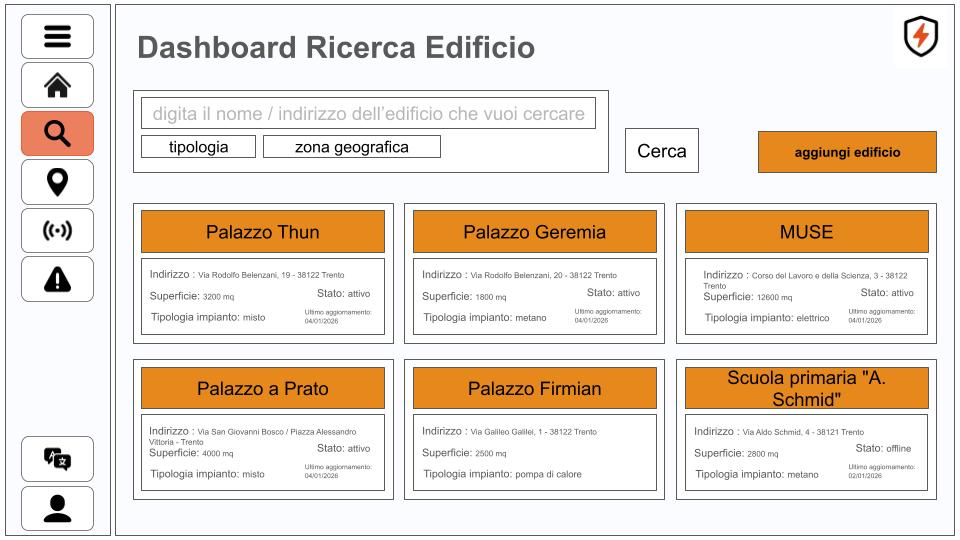
\includegraphics[width=1\textwidth]{../images/Interfaccia_grafica/Pannello_Ricerca.jpg}
    \caption{Dashboard Ricerca Edificio}
    \label{fig:ricerca_edificio}
\end{figure}

La Figura~\ref{fig:ricerca_edificio} illustra la schermata di consultazione e ricerca del patrimonio edilizio censito nel sistema.

\begin{itemize}
    \item \textbf{RF3: Ricerca edifici}
    \begin{itemize}
        \item L'utente ha a disposizione una barra di testo libero per cercare per nome o indirizzo, affiancata da menu a tendina per filtrare per "tipologia" e "zona geografica", con pulsante "Cerca". I risultati restituiti sotto forma di schede mostrano le informazioni chiave dell'edificio: indirizzo, superficie in $\text{m}^2$, tipologia dell'impianto termico, stato operativo (attivo o offline) e timestamp dell'ultimo aggiornamento dati.
    \end{itemize}

    \item \textbf{RF5: Gestione edifici}
    \begin{itemize}
        \item Nella parte superiore della vista è integrato il pulsante rapido "aggiungi edificio", tramite il quale gli operatori e gli amministratori abilitati possono censire una nuova struttura all'interno della piattaforma inserendone i dati anagrafici.
    \end{itemize}

    \item \textbf{RNF2: Performance}
    \begin{itemize}
        \item L'impostazione dei criteri di filtro combinabili e la struttura a schede sintetiche sono progettate per garantire l'elaborazione dei parametri e la restituzione dell'elenco degli edifici entro il vincolo prestazionale dei 5 secondi prefissato nei requisiti.
    \end{itemize}
\end{itemize}

\subsection{Dashboard Mappa Edifici}
\begin{figure}[H]
    \centering
    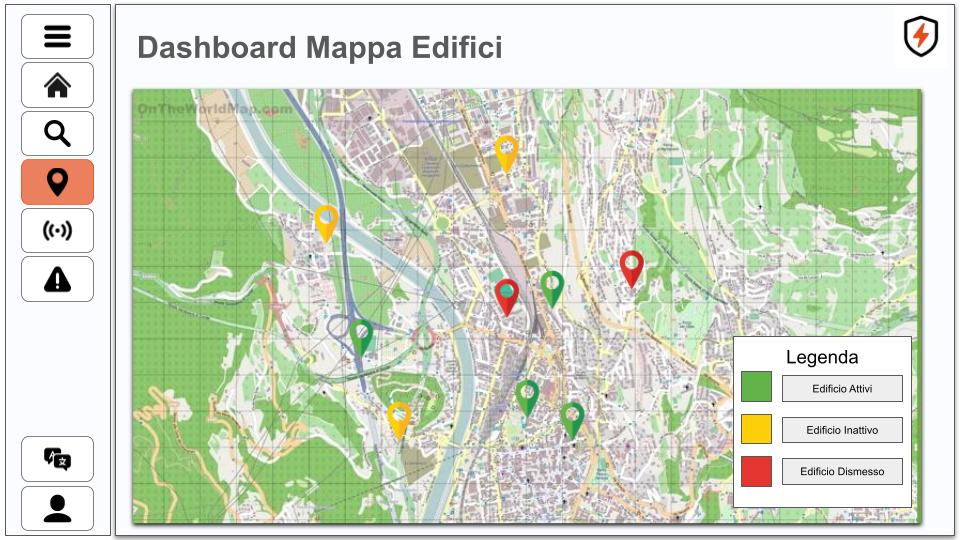
\includegraphics[width=1\textwidth]{../images/Interfaccia_grafica/Mappa.jpg}
    \caption{Dashboard Mappa Edifici}
    \label{fig:mappa_edifici}
\end{figure}

La Figura~\ref{fig:mappa_edifici} presenta la vista geografica interattiva del patrimonio edilizio comunale, consentendo agli operatori e agli amministratori una navigazione territoriale intuitiva e georeferenziata.

\begin{itemize}
    \item \textbf{RF3: Ricerca edifici (Localizzazione cartografica)}
    \begin{itemize}
        \item Il sistema integra una mappa del territorio comunale su cui sono posizionati dei marker interattivi in corrispondenza delle coordinate geografiche di ciascuna struttura pubblica, consentendo l'identificazione spaziale immediata degli stabili censiti.
    \end{itemize}

    \item \textbf{RF5: Gestione edifici (Stato operativo sul territorio)}
    \begin{itemize}
        \item I marker cartografici riflettono visivamente lo stato operativo dell'edificio mediante una codifica cromatica formalizzata nella legenda a schermo: verde per "Edificio Attivo", giallo per "Edificio Inattivo" e rosso per "Edificio Dismesso".
    \end{itemize}

\end{itemize}

\newpage

\subsection{Dashboard Gestione Allarmi}
\begin{figure}[H]
    \centering
    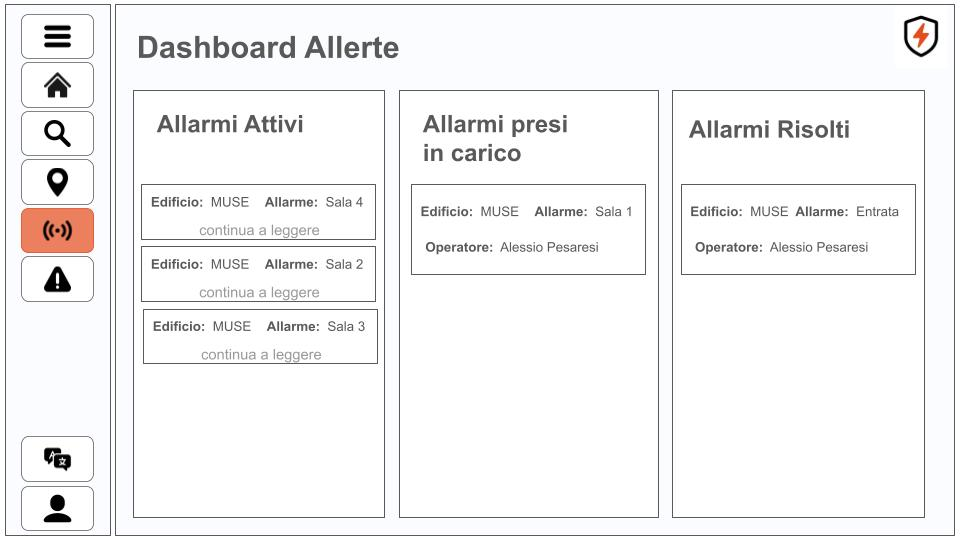
\includegraphics[width=1\textwidth]{../images/Interfaccia_grafica/Allerte.jpg}
    \caption{Dashboard Gestione Allarmi}
    \label{fig:allarmi}
\end{figure}

La Figura~\ref{fig:allarmi} mostra il pannello dedicato al controllo, alla gestione e alla presa in carico delle notifiche di anomalia generate dal superamento delle soglie impostate sui sensori.

\begin{itemize}
    \item \textbf{RF6: Gestione notifiche di allarme}
    \begin{itemize}
        \item Le segnalazioni sono organizzate in un pannello strutturato a tab che ne traccia l'intero ciclo di vita: "Allarmi Attivi", "Allarmi presi in carico" e "Allarmi Risolti". Per ogni segnalazione viene riportato l'edificio coinvolto (es. \textit{MUSE}), la posizione specifica del sensore (Sala 1, Sala 2, Sala 4, Entrata), l'eventuale operatore assegnato alla gestione dell'evento (es. Alessio Pesaresi) e il comando rapido per consultare i dettagli completi dell'allerta.
    \end{itemize}

    \item \textbf{RF9: Configurazione soglie di allarme (Monitoraggio eventi)}
    \begin{itemize}
        \item La presenza delle notifiche in elenco riflette l'avvenuta violazione delle soglie minime o massime precedentemente configurate per i parametri ambientali o energetici dei sensori.
    \end{itemize}

\end{itemize}

\newpage

\subsection{Dashboard Stato Sensori}
\begin{figure}[H]
    \centering
    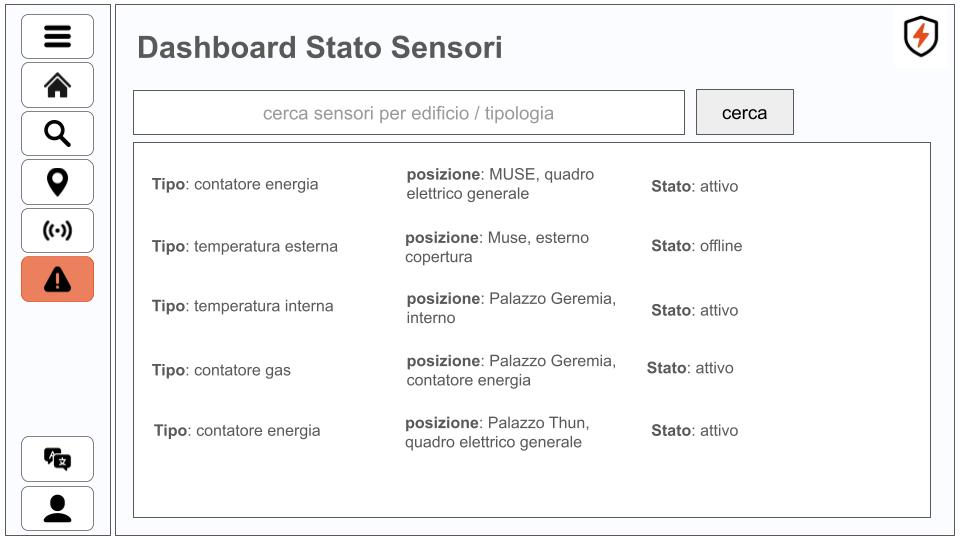
\includegraphics[width=1\textwidth]{../images/Interfaccia_grafica/Sensori.jpg}
    \caption{Dashboard Stato Sensori}
    \label{fig:stato_sensori}
\end{figure}

La Figura~\ref{fig:stato_sensori} illustra la schermata riepilogativa dedicata all'infrastruttura IoT e alla telemetria, fornendo una diagnostica continua sui dispositivi installati negli edifici.

\begin{itemize}
    \item \textbf{RF3: Ricerca sensori}
    \begin{itemize}
        \item Nella parte superiore è presente una barra di ricerca dedicata (\textit{"cerca sensori per edificio / tipologia"}) con pulsante \textit{"cerca"}, che permette di isolare e filtrare rapidamente specifici componenti hardware o aree dell'impianto.
    \end{itemize}
    
    \item \textbf{RF7: Visualizzazione stato sensori}
    \begin{itemize}
        \item L'interfaccia espone l'elenco tabellare di tutti i dispositivi presenti negli edifici comunali (contatori di energia elettrica, contatori di gas, sonde di temperatura interna ed esterna), specificandone per ciascuno la tipologia, la collocazione fisica precisa (es. \textit{MUSE, quadro elettrico generale}; \textit{Palazzo Geremia, interno}) e lo stato operativo corrente (attivo o offline).
    \end{itemize}

    \item \textbf{RNF4: Affidabilità}
    \begin{itemize}
        \item Lo stato "offline" dei dispositivi non raggiungibili (es. sonda di temperatura esterna del MUSE) viene evidenziato chiaramente, permettendo al personale tecnico di programmare tempestivamente gli interventi di manutenzione fisica o di ripristino della connettività.
    \end{itemize}
\end{itemize}

\newpage

\subsection{Dashboard Utenti}
\begin{figure}[H]
    \centering
    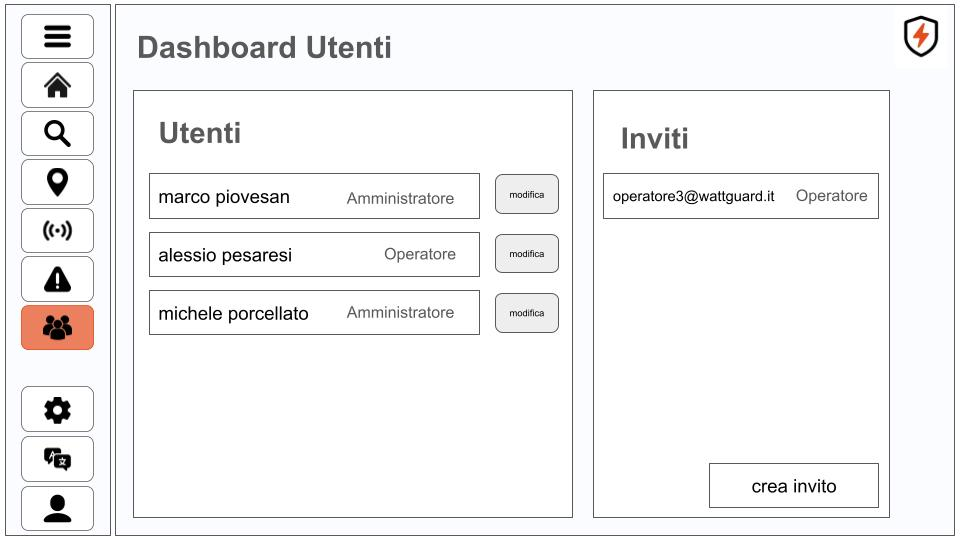
\includegraphics[width=1\textwidth]{../images/Interfaccia_grafica/Utenti.jpg}
    \caption{Dashboard Gestione Utenti}
    \label{fig:gestione_utenti}
\end{figure}

La Figura~\ref{fig:gestione_utenti} mostra la schermata riservata all'Amministratore comunale per l'amministrazione delle autorizzazioni e la gestione degli account della piattaforma.

\begin{itemize}
    \item \textbf{RF11: Gestione utenti (Funzionalità esclusiva Amministratore)}
    \begin{itemize}
        \item Il pannello consente la completa gestione delle utenze: nella sezione superiore "Utenti" elenca i nominativi attivi con il rispettivo livello di privilegio (Amministratore o Operatore) e offre il pulsante "modifica" per aggiornare i ruoli o revocare l'accesso. La sezione "Inviti" permette di abilitare nuovi utenti specificando l'indirizzo email (es. \textit{operatore3@wattguard.it}) e il ruolo, inviando una notifica automatica con token univoco tramite il comando "crea invito".
    \end{itemize}

    \item \textbf{RNF5: Sicurezza (Role-Based Access Control)}
    \begin{itemize}
        \item L'accesso a questa schermata è rigorosamente limitato agli utenti con ruolo di amministratore, garantendo la segregazione dei poteri applicativi e il controllo centralizzato sul ciclo di vita delle credenziali.
    \end{itemize}
\end{itemize}

\newpage

\subsection{Impostazioni di Sistema}
\begin{figure}[H]
    \centering
    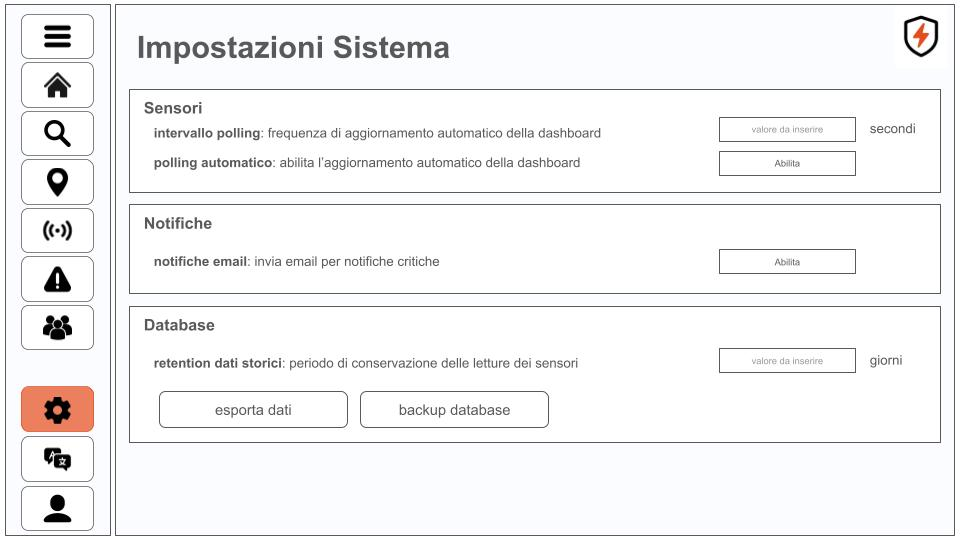
\includegraphics[width=1\textwidth]{../images/Interfaccia_grafica/Impostazioni.jpg}
    \caption{Pannello Impostazioni di Sistema}
    \label{fig:impostazioni_sistema}
\end{figure}

La Figura~\ref{fig:impostazioni_sistema} illustra il modulo di configurazione dei parametri globali della piattaforma, delle frequenze di telemetria e delle procedure di salvaguardia dei dati.

\begin{itemize}
    \item \textbf{RF8: Monitoraggio tempo reale (Configurazione frequenze)}
    \begin{itemize}
        \item Nella sezione "Sensori" è possibile impostare l'"intervallo polling" (specificando il valore numerico in secondi) e abilitare o sospendere l'aggiornamento automatico dei flussi mediante il controllo dedicato "polling automatico".
    \end{itemize}

    \item \textbf{RF9: Configurazione soglie di allarme e notifiche}
    \begin{itemize}
        \item La sezione "Notifiche" include lo switch "notifiche email" per abilitare l'inoltro automatico di avvisi di posta elettronica in presenza di superamento dei limiti di soglia o anomalie critiche.
    \end{itemize}

    \item \textbf{RF10: Esportazione dati (Funzionalità esclusiva Amministratore)}
    \begin{itemize}
        \item È presente il pulsante rapido "esporta dati", che consente all'amministratore di estrarre le serie storiche dei rilievi e delle anomalie nei formati standard previsti (CSV, Excel, PDF).
    \end{itemize}
    
    \item \textbf{RNF2: Performance}
    \begin{itemize}
        \item La possibilità di regolare la frequenza di polling permette agli amministratori di calibrare il bilanciamento tra tempestività dei dati e carico generato sul server e sulla rete.
    \end{itemize}
    \newpage
    \item \textbf{RNF4: Affidabilità e persistenza}
    \begin{itemize}
        \item L'interfaccia permette di impostare la "retention dati storici" definendo il periodo minimo di conservazione delle misurazioni in giorni (con vincolo minimo di 1 giorno) e mette a disposizione il comando "backup database" per esportare un dump integrale dei dati in formato JSON escludendo le informazioni sensibili.
    \end{itemize}

\end{itemize}